\section{Introduction}

In this document, we formalize a method for pruning infeasible paths from control-flow 
graphs. The method formalized here is a graph-transformation approach based on \emph{symbolic 
execution}. Since we consider programs with unbounded loops, symbolic execution
is augmented by the 
detection of \emph{subsumptions} in order to stop unrolling loops eventually. The method follows the 
\emph{abstract-check-refine} paradigm. Abstractions are allowed in order to force 
subsumptions. But, since abstraction consists of loosing part of information at a given point, 
abstractions might introduce infeasible paths into the result. A counterexample guided refinement 
is used to rule out such abstractions. 

This method takes a CFG $G$ and a user given precondition and builds a new CFG $G'$ that still 
over-approximates the set of feasible paths of $G$ but contains less infeasible paths. 
It proceeds basically as follows (see~\cite{AGVW2016} for more details). 
First, it starts by building a classical symbolic execution tree (SET) of the program under analysis. 
As soon as a cyclic path is detected, the algorithm searches for a subsumption of the point at the 
end of the cycle by one of its ancestors. When doing this, the algorithm is allowed to abstract 
the ancestor in order to force the subsumption. When a subsumption is established, the current 
symbolic execution halts along that path and a subsumption link is added to the SET, turning it into 
a symbolic execution graph (SEG). When an occurrence of a final location of the original CFG 
is reached, we check if abstractions that might have been performed along the current path did not 
introduce certain infeasible paths in the new representation. If no refinement is needed, symbolic 
execution resumes at the next pending point. Otherwise, the analysis restarts at the point where the 
``faulty'' abstraction occurred, but now this point is strengthened with a \emph{safeguard 
condition}: future abstractions occurring at this point will have to entail the safeguard 
condition, preventing the faulty abstraction to occur again. These safeguard conditions could be 
user-provided but are typically the result of a \emph{weakest precondition calculus}. When the 
analysis is over, the SEG is turned into a new CFG.

Our motivation is in random testing of imperative programs. There exist efficient algorithms that 
draw in a statistically uniform way long paths from very large graphs~\cite{Denise2011}. If the 
probability of drawing a feasible path from such a transformed CFG was high, this would lead to an 
efficient statistical structural white-box testing method. With testing in mind, a crucial 
property that our approach must have, besides being correct, is to preserve the set of feasible 
paths of the original CFG. Our goal with this formalization is to establish correctness of the 
approach and the fact that it preserves the feasible paths of the original CFG, that is:
\begin{enumerate}
  \item for every path in the new CFG, there exists a path with the same trace in the original CFG,
  \item for every feasible path of the original CFG, there exists a path with the same trace in 
the new CFG.
\end{enumerate}

We consider that our method is made of five graph-transformation operators and a set of 
heuristics. These five operators consist in:
\begin{enumerate}
  \item adding an arc to the SEG as the result of a symbolic execution step in the
    original CFG,
  \item adding a subsumption link to the SEG,
  \item abstracting a node of the SEG,
  \item marking a node as unsatisfiable,
  \item labelling a node with a safeguard condition.
\end{enumerate} 
Heuristics control, for example, the order in which these operators
are applied, which of the possible
abstractions is selected, etc. These heuristics cannot interfer with the 
correctness of the approach or the preservation of feasible paths since they
simply combine the five kernel transformations. In the following, 
we model the different data structures that our method performs on and formalize our five 
operators but completely skip the heuristics aspects of the approach. Thus, our results extend to a 
large family of algorithms that add specific heuristics in their goal to over-approximate the 
set of feasible paths of a CFG.

Due to the nature of the problem, symbolic execution in presence of unbounded loops, such algorithms 
might not terminate. In practice, this is handled using some kind of timeout condition. When such 
condition triggers, the SEG is only a partial unfolding of the original CFG. Thus, the resulting 
CFG cannot contains all feasible paths of the original one. In this situation, the only way to 
preserve the set of feasible paths is to ``connect'' the SEG to the original CFG. The SEG is the currently 
known over-approximating set of prefixes of feasible paths and the original CFG represents the 
unknown part of the set of feasible paths. 

In the following, we use an adequate data structure that 
we call a \emph{red-black graph}. Its \emph{black part} is the original CFG: it represents 
the unknown part of the set of feasible paths and is never modified during the analysis. The 
\emph{red part} represents the SEG: its vertices are occurrences of the vertices of the black part. 
Then, we define the five operators that will modify the red part 
as described previously. We only consider red-black graphs built using these five operators, 
starting from a red-black graph whose red part is empty. Paths of such structures are called 
\emph{red-black paths}. Such paths start in the red part and might end in the black part: they 
are made of a red feasible prefix and a black prefix on which nothing is known about feasibility.
Finally, we prove that, given any red-black graph built using our five operators and modulo a 
renaming of vertices, the set of red-black paths is a subset of the set of black paths and that 
the set of feasible black paths is a subset of the set of red-black paths. 

In the following, we proceed as follows (see Figure~\ref{fig:theory_hierarchy} for the detailed hierarchy). First, we formalize all the aspects related to symbolic 
execution, subsumption and abstraction (\verb?Aexp.thy?, \verb?Bexp.thy?, \verb?Store.thy?, 
\verb?Conf.thy?, \verb?Labels.thy?, 
\verb?SymExec.thy?). Then, we formalize graphs and their paths (\verb?Graph.thy?). Using extensible records allows 
us to model Labeled Transition Systems from graphs (\verb?Lts.thy?). Since we are 
interested in paths going through subsumption links, we also define these notions for graphs equipped 
with subsumption relations (\verb?SubRel.thy?) and prove a number of theorems describing how the 
set of paths of such graphs evolve when an arc (\verb?ArcExt.thy?) or a subsumption link 
(\verb?SubExt.thy?) is 
added. Finally, we formalize the notion of red-black graphs and prove the two 
properties we are mainly interested in (\verb?RB.thy?).

\begin{figure*}
	\centering
	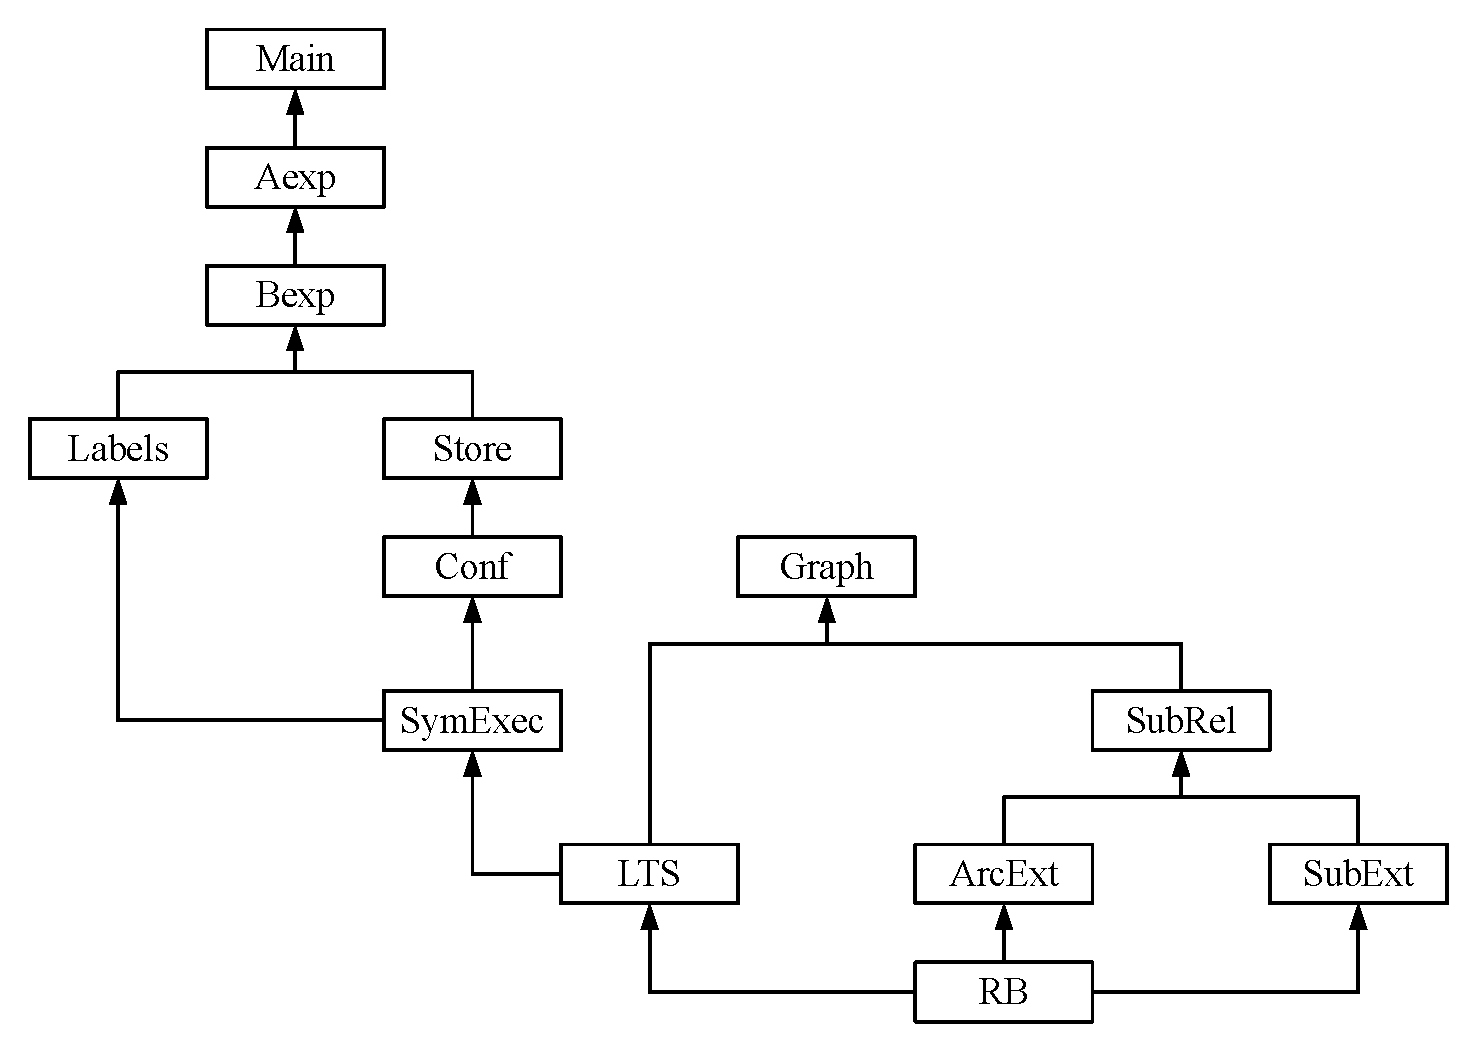
\includegraphics[scale=.5]{theory_hierarchy}
	\caption{The hierarchy of theories.}
	\label{fig:theory_hierarchy}
\end{figure*}
